\documentclass{article}
\usepackage[top=3.2cm,bottom=3.2cm,right=2.5cm,left=2.5cm]{geometry}
\usepackage[x11names, rgb]{xcolor}
\usepackage[utf8]{inputenc}
\usepackage{tikz}
\usepackage[urw-garamond]{mathdesign}
\usetikzlibrary{snakes,arrows,shapes}
\usepackage{amsmath}
%
%

%

%

\begin{document}
\pagestyle{empty}
%
%
%

% Start of code
\begin{center}
{\Large \bfseries Project Nemaload Breakdown}
\vfill
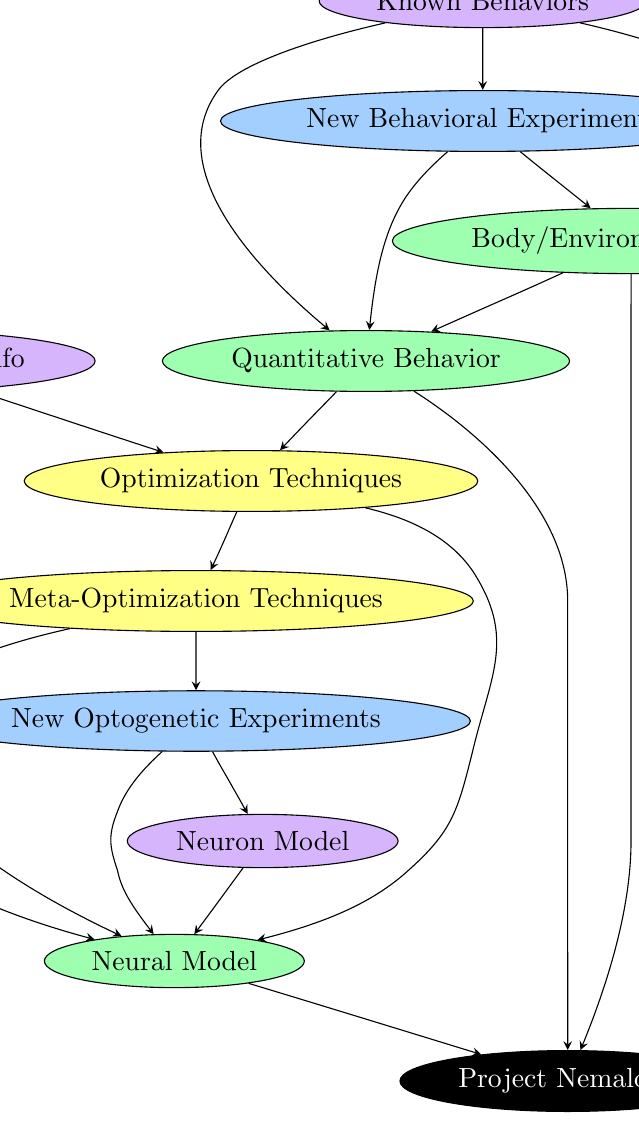
\begin{tikzpicture}[scale=0.6,>=stealth,line join=bevel]
%%
\definecolor{fillcolor}{rgb}{1.0,1.0,0.52};
  \path[use as bounding box] (200bp,0bp) rectangle (550bp,650bp);
  \node (opt) at (334bp,378bp) [draw,fill=fillcolor,ellipse] {Optimization Techniques};
  \definecolor{fillcolor}{rgb}{0.64,0.81,1.0};
  \node (new_behav) at (473bp,594bp) [draw,fill=fillcolor,ellipse] {New Behavioral Experiments};
  \definecolor{fillcolor}{rgb}{1.0,1.0,0.52};
  \node (metaopt) at (301bp,306bp) [draw,fill=fillcolor,ellipse] {Meta-Optimization Techniques};
  \definecolor{fillcolor}{rgb}{0.64,0.81,1.0};
  \node (opto) at (301bp,234bp) [draw,fill=fillcolor,ellipse] {New Optogenetic Experiments};
  \definecolor{fillcolor}{rgb}{0.62,1.0,0.69};
  \node (quant_behav) at (403bp,450bp) [draw,fill=fillcolor,ellipse] {Quantitative Behavior};
  \definecolor{fillcolor}{rgb}{0.84,0.71,0.99};
  \node (known_behav) at (473bp,666bp) [draw,fill=fillcolor,ellipse] {Known Behaviors};
  \definecolor{fillcolor}{rgb}{0.62,1.0,0.69};
  \node (env_model) at (562bp,522bp) [draw,fill=fillcolor,ellipse] {Body/Environment Model};
  \definecolor{fillcolor}{rgb}{0.62,1.0,0.69};
  \node (neural_model) at (288bp,90bp) [draw,fill=fillcolor,ellipse] {Neural Model};
	\node (nemaload) at (524bp,18bp) [draw,fill=black,ellipse] {\color{white} Project Nemaload};
  \definecolor{fillcolor}{rgb}{0.84,0.71,0.99};
  \node (white) at (115bp,450bp) [draw,fill=fillcolor,ellipse] {Existing Topology Info};
  \definecolor{fillcolor}{rgb}{0.84,0.71,0.99};
  \node (neuron_model) at (341bp,162bp) [draw,fill=fillcolor,ellipse] {Neuron Model};
  \draw [->] (neuron_model) ..controls (322bp,136bp) and (314bp,125bp)  .. (neural_model);
  \draw [->] (env_model) ..controls (562bp,476bp) and (562bp,423bp)  .. (562bp,378bp) .. controls (562bp,378bp) and (562bp,378bp)  .. (562bp,162bp) .. controls (562bp,120bp) and (547bp,74bp)  .. (nemaload);
  \draw [->] (env_model) ..controls (502bp,494bp) and (474bp,482bp)  .. (quant_behav);
  \draw [->] (quant_behav) ..controls (468bp,409bp) and (524bp,362bp)  .. (524bp,306bp) .. controls (524bp,306bp) and (524bp,306bp)  .. (524bp,162bp) .. controls (524bp,122bp) and (524bp,75bp)  .. (nemaload);
  \draw [->] (opt) ..controls (322bp,352bp) and (318bp,342bp)  .. (metaopt);
  \draw [->] (white) ..controls (197bp,423bp) and (239bp,409bp)  .. (opt);
  \draw [->] (known_behav) ..controls (371bp,643bp) and (325bp,628bp)  .. (314bp,612bp) .. controls (281bp,566bp) and (335bp,507bp)  .. (quant_behav);
  \draw [->] (quant_behav) ..controls (377bp,423bp) and (367bp,413bp)  .. (opt);
  \draw [->] (opto) ..controls (270bp,206bp) and (259bp,194bp)  .. (254bp,180bp) .. controls (248bp,165bp) and (249bp,159bp)  .. (254bp,144bp) .. controls (256bp,134bp) and (261bp,125bp)  .. (neural_model);
  \draw [->] (new_behav) ..controls (441bp,566bp) and (429bp,554bp)  .. (422bp,540bp) .. controls (412bp,521bp) and (408bp,497bp)  .. (quant_behav);
  \draw [->] (known_behav) ..controls (473bp,640bp) and (473bp,631bp)  .. (new_behav);
  \draw [->] (new_behav) ..controls (506bp,567bp) and (520bp,556bp)  .. (env_model);
  \draw [->] (white) ..controls (96bp,405bp) and (78bp,352bp)  .. (78bp,306bp) .. controls (78bp,306bp) and (78bp,306bp)  .. (78bp,234bp) .. controls (78bp,162bp) and (162bp,124bp)  .. (neural_model);
  \draw [->] (known_behav) ..controls (575bp,643bp) and (620bp,628bp)  .. (632bp,612bp) .. controls (641bp,598bp) and (639bp,590bp)  .. (632bp,576bp) .. controls (626bp,564bp) and (616bp,554bp)  .. (env_model);
  \draw [->] (metaopt) ..controls (301bp,280bp) and (301bp,271bp)  .. (opto);
  \draw [->] (metaopt) ..controls (187bp,281bp) and (146bp,267bp)  .. (135bp,252bp) .. controls (95bp,196bp) and (184bp,139bp)  .. (neural_model);
  \draw [->] (opto) ..controls (315bp,208bp) and (321bp,198bp)  .. (neuron_model);
  \draw [->] (opt) ..controls (432bp,355bp) and (454bp,343bp)  .. (467bp,324bp) .. controls (493bp,284bp) and (478bp,262bp)  .. (467bp,216bp) .. controls (458bp,180bp) and (455bp,168bp)  .. (428bp,144bp) .. controls (407bp,125bp) and (379bp,113bp)  .. (neural_model);
  \draw [->] (neural_model) ..controls (371bp,65bp) and (423bp,49bp)  .. (nemaload);
%
\end{tikzpicture}
\end{center}
% End of code
\vspace*{\stretch{1}}
{\large \bfseries Legend \\\rule[5mm]{5cm}{1.0pt}\\}
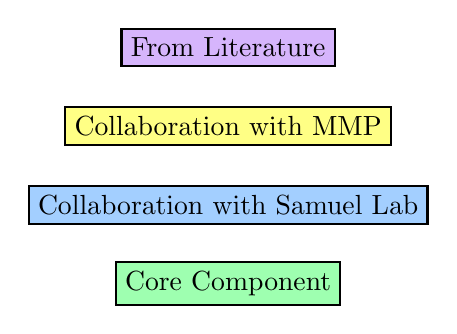
\begin{tikzpicture}[outline/.style={draw=black,thick,fill=#1}]
  \definecolor{core}{rgb}{0.62,1.0,0.69};
  \definecolor{samuel}{rgb}{0.64,0.81,1.0};
  \definecolor{mmp}{rgb}{1.0,1.0,0.52};
  \definecolor{lit}{rgb}{0.84,0.71,0.99};
	\node [outline=core] at (0,0) {Core Component};
	\node [outline=samuel] at (0,1) {Collaboration with Samuel Lab};
	\node [outline=mmp] at (0,2) {Collaboration with MMP};
	\node [outline=lit] at (0,3) {From Literature};
\end{tikzpicture}



%
\end{document}
%


